\chapter{Practice: Blinking LED}\label{pract:blinkingLED}
\section*{Suggested read: Chapers~\ref{introToArduino}~and~\ref{pract:settingTheIDE}}

In the following practice you will write your first Arduino application. Although simple, mastering it will provide you with clear understanding of the IDE and the components that conform the Arduino platform.

It consist of a simple code that will turn on/off LED(s) plugged to the digital IO ports of the Arduino.

\section{Preparing your development environment}
For Practice~\ref{pract:blinkingLED}, you will need:
\begin{itemize}
 \item as many LEDs as you want, but always less than the number of digital IO ports.
 \item a USB cable to connect your Arduino board to the PC.
 \item the Arduino IDE, up and running.
\end{itemize}

Turn your Arduino on by plugging it to the PC. Make sure you have selected the appropriate COM port, as it is explained in Practice~\ref{pract:settingTheIDE} according with your operating system.

\section{The code} 
Once inside, enter the following code:

\begin{lstlisting} [caption = {Blinking LED example code}, language = C, label = {code:blinkingLED}, numbers = left, escapeinside={@}{@}]
const int LED = 13; @\label{BL:LED}@

void setup() @\label{BL:SETUP}@
{
	pinMode(LED,OUTPUT); @\label{BL:pinMODE}@
}

void loop() @\label{BL:LOOP}@
{
	digitalWrite(LED, HIGH); @\label{BL:HIGH}@
	delay(1000); @\label{BL:DELAY}@
	digitalWrite(LED, LOW); @\label{BL:LOW}@
	delay(1000); @\label{BL:DELAY2}@
}
\end{lstlisting}

As you might be able to see, the code is completely readable. Let's review it line by line.

\begin{itemize}
	\item Line~\ref{BL:LED}: \texttt{const int LED = 13}, assigns the value $13$ to a \texttt{\color{red}{int}}erger variable, named LED. In this case, this number corresponds to the digital IO port \#13.
	\item Line~\ref{BL:SETUP}: \texttt{void setup()} is the name of the next block of code. It is very similar to functions in languages like C/C++ and it is generally used to assign variables to ports, as well as their role.
	\item Line~\ref{BL:pinMODE}: \texttt{pinMode(LED,OUTPUT)} tells the Arduino how to set the pins. In this case, pin LED ($\#13$) is set up as an OUTPUT. \texttt{pinMode} is a function, and the words or numbers inside the parenthesis are its arguments.
	\item Line~\ref{BL:LOOP}: \texttt{void loop()}: is where you define the behaviour of your device. The statements contained in \texttt{loop()} are repeated over and over again until the device is turned off.
	\item Line~\ref{BL:HIGH}: \texttt{digitalWrite(LED, HIGH)} works as a power socket for pins. In this case, the command is indicating to turn pin \texttt{LED} into \texttt{HIGH}, which instructs Arduino to turn the output pin to $5$V. If you have connected a LED in this pin, the result is that it will turn on (hopefully). Turning on and off the pin allow us to see what the software is making the hardware do; the LED is an actuator.
	\item Line~\ref{BL:DELAY}: \texttt{delay(1000)} tells the processor to wait for $1000$ \emph{milliseconds} before proceeding to the next code line.
	\item Line~\ref{BL:LOW}: \texttt{digitalWrite(LED, LOW)} as with Line~\ref{BL:HIGH}, this function turns pin \texttt{LED} to $0$V, causing the connected LED to turn off. You can do a mental map in which $HIGH \rightarrow ON,\ LOW \rightarrow OFF$.
	\item Line~\ref{BL:DELAY2}: because the last instruction was to set the LED off, this will keep it that way for an additional $1000$ \emph{millisecods}.
\end{itemize}

To see your work, just insert the longer leg of the LED into the digital IO port you assigned to variable \texttt{LED} on your code (digital pin $13$), and the shorter leg to ground (GND). Figure~\ref{fig:blinkingLEDLayout} shows the desired layout.

\begin{figure}[htbp]
  \centering
  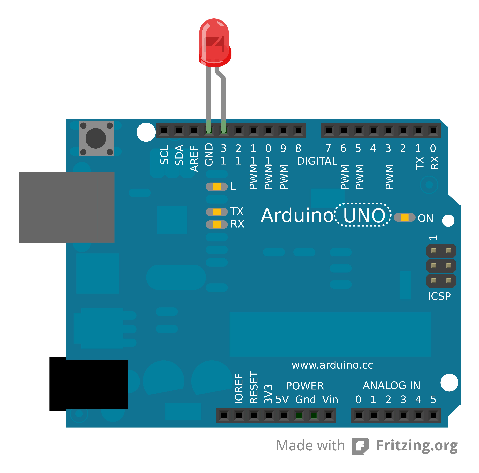
\includegraphics[width=0.7\linewidth]{figures/blinkingLED-NEW.eps}
  \caption{Blinking LED layout
  \label{fig:blinkingLEDLayout}}
\end{figure}
